\chapter{Der Photoeffekt}
%Some parts will be used later

%Die Grundlagen werden später gelöscht und der Inhalt in die Durchführung/Auswertung eingebaut
%\section{Grundlagen}
%\subsection{Photoeffekt}
%Der Photoeffekt tritt bei Ionisierung von Atomen durch Lichteinstrahlung, wobei die Energie der Valenzelektronen so weit ansteigt, dass sie das Potential des Atoms verlassen können. Dies geschieht nur, wenn das Licht eine Mindestenergie erreicht, die der Tiefe des Elektronenpotentials entspricht. Die Energie des Lichts \(E\) hängt mit ihrer Frequenz \(\nu\) durch die Beziehung \(E = \nu h\) zusammen, wobei \(h\) das Plancksche Wirkungsquantum darstellt. 
%\subsection{Funktionsweise einer Photozelle}

%\paragraph{Aufbau}
%Eine Photozelle besteht aus einer Ringanode und einer Kathode, welche mit Licht beleuchtet
%wird. Die Anode und die Kathode bestehen aus unterschiedlichen Materialien.


%\begin{figure}[htbp]
%    \centering
%    \includegraphics[width=0.75\textwidth]{figs/anlegen_aeuß_potential.png}
%    \caption{ Kontaktpotential $-eU_{KA}$ \cite{praktikum}}
%    \label{fig:potential ext}
%\end{figure}
%\FloatBarrier

%\begin{figure}[htbp]
%    \centering
%    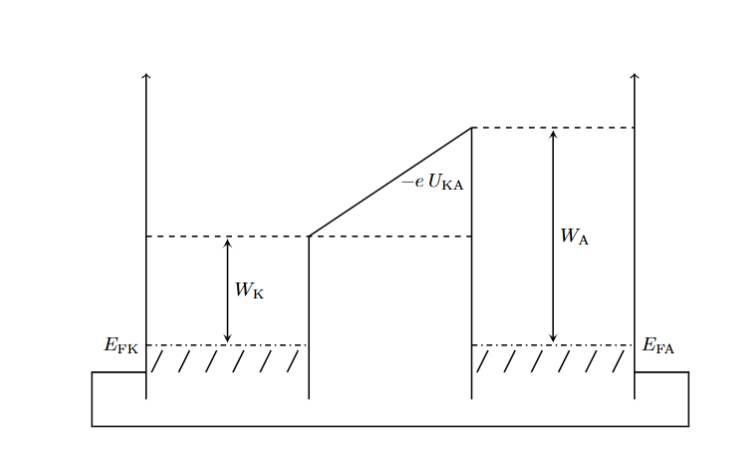
\includegraphics[width=0.75\textwidth]{figs/kontaktpotential_kurzgeschl_elektroden.png}
%    \caption{  Potential dass von der Gegenspannung
%$-eU_G$ induziert wird\cite{praktikum}}
%    \label{fig:potential kurzg.}
%\end{figure}
%\FloatBarrier

%\paragraph{Wirkung}
%\begin{figure}[htbp]
%    \centering
%    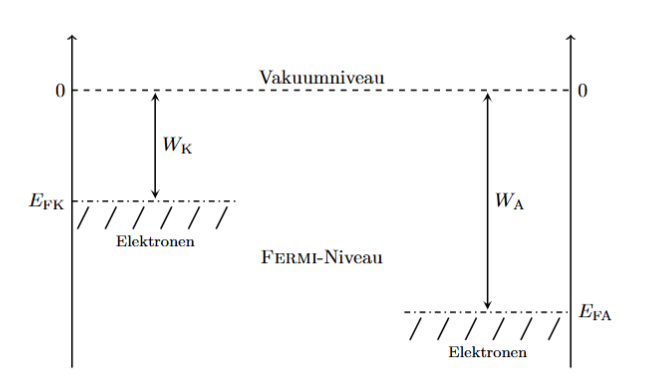
\includegraphics[width=0.75\textwidth]{figs/baenderschema_kathode_anode.png}
%    \caption{ Ferminiveaus von Kathode und Anode mit Austrittsarbeit $W_A$ \cite{praktikum}}
%    \label{fig:kathode-anode}
%\end{figure}
%\FloatBarrier
%Das Anodenmaterial weist eine höhere Austrittsarbeit auf als das Kathodenmaterial, wodurch beim Kontakt eine Potentialdifferenz zwischen ihren Ferminiveaus entsteht. Diese Differenz verstärkt sich, wenn eine zusätzliche Gegenspannung zwischen Anode und Kathode angelegt wird.\\
%Die durch das Licht herausgelösten Elektronen gewinnen entsprechend seiner Energie kinetische Energie und bewegen sich zur Anode, wodurch ein messbarer Strom entsteht. Die angelegte Gegenspannung verlangsamt die Elektronen und wird schrittweise erhöht, bis kein Photostrom mehr nachweisbar ist – also die Elektronen aus dem Anodenmaterial nicht mehr die Anode erreichen.
%\paragraph{Photostromverlauf}
%\paragraph{Austrittsarbeit}
%\paragraph{Kontaktpotential}




%bleibt da, den Aufbau erläutern
\section{Aufbau}
\begin{figure}[htbp]
    \centering
    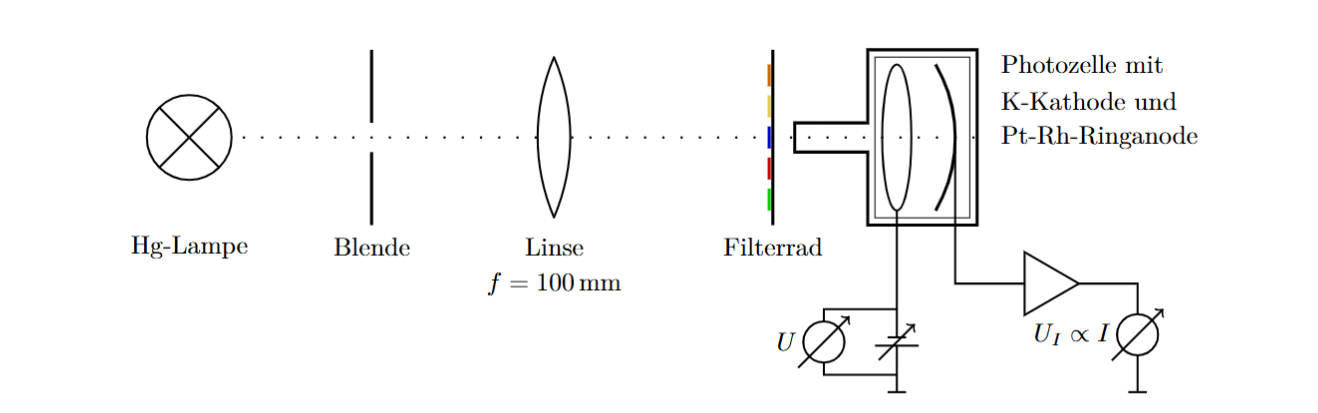
\includegraphics[width=0.75\textwidth]{figs/Aufbau_plank_wirkungsquantum.png}
    \caption{Aufbau für die Messung des Photoeffektes  \cite{praktikum}}
    \label{fig:aufbau teil 1}
\end{figure}
\FloatBarrier
Links ist die Hg-Lampe zu sehen, in der
Mitte Optik-Elemente zum Fokussieren und Filtern des Lichtes und rechts ist die Photozelle
mit Gegenspannung und Strommessung.\\
Die Quecksilber-Spektrallampe und die Photozelle 
werden gemäß Abbildung \ref{fig:aufbau teil 1} 
gegenüberliegend auf dem Reiter angeordnet. 
Eine Irisblende vor der Lampe ermöglicht die 
Regulierung der Lichtintensität. Eine Linse 
mit einer Brennweite von f=100 mm wird in 
diesem Abstand vor die Blende positioniert,
 sodass sie das Licht parallel auf den 
 nachfolgenden Interferenzfilter mit fünf 
 Filtern sowie eine zusätzliche Blende lenkt.

%---------------------------------------------------------------
\section{Durchführung}

Eine Abschirmvorrichtung mit einem 
röhrenförmigen Element verhindert Streulicht. 
Ein Lichtfleck wird gezielt auf die Kathode 
projiziert, ohne ,dass die Anode beleuchtet wird.

Wenn Photonen aus der Hg-Lampe auf die Photokathode treffen, interagieren sie mit den Elektronen in dieser und überträgt dabei seine gesamte Energie $E = h\nu$
auf eines der Elektronen. Falls die übertragene Energie größer als die Austrittsarbeit $W_A$ ist,dann kann sich das Elektron aus der Kathode lösen und zur Ringanode gelangen. Dadurch ensteht ein Stromfluss:der Photostrom $I_{ph}$.
Durch den Einsatz der Gegenfeldmethode wird die maximale kinetische Energie, die die Elektronen beim verlassen der Kathode besitzen, bestimmt.

Bei dieser Methode wird eine Gegenspannung $U_G$ zwischen Kathode und Anode angelegt, wodurch die Kathode im Vergleich zur Anode ein positives Potential erhält.
Das dadurch erzeugte elektrische Feld verlangsamt die emittierten Elektronen auf ihrem Weg zur Anode, wodurch der Photostrom reduziert wird. Sobald die Grenzspannung $U_0$ erreicht ist, kommt der Photostrom vollständig zum Erliegen. 
Dies bedeutet, dass selbst die energiereichsten Elektronen die Anode nicht mehr erreichen können. In diesem Fall gilt die Beziehung: 
$E_{kin,max} = eU_0$.

Man lässt das Gegenfeld mit Hilfe einer variablen Spannungsquelle, welche sich zwischen der Kathode und der Anode befindet, ansteigen.
Man erweitert die Schaltung mit Hilfe eines Spannungsteilers (Abbildung \ref{fig:spannungsteiler}) aus einem $330\Omega$ und $100\Omega$ Widerstandes um den Messbereich zu skalieren und genauere Messungen durchzuführen.
\begin{figure}[htbp]
    \centering
    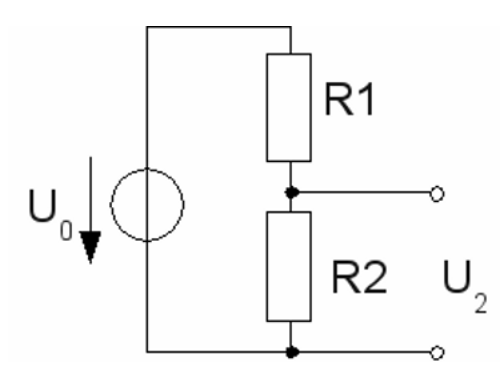
\includegraphics[width=0.3\textwidth]{figs/Spannungsteiler.png}
    \caption{ Spannungsteiler \cite{Spannungsteiler}}
    \label{fig:spannungsteiler}
\end{figure}
\FloatBarrier
Die verwendete Spannungsquelle kann Spannungen von 0\,V bis 12\,V bereitstellen. 
Der Photostrom erreicht jedoch bereits bei deutlich geringeren Gegenspannungen seinen Nullpunkt, typischerweise im Bereich von wenigen Volt. 
Für die Messung der Grenzspannung $U_0$ genügt daher ein kleiner Teil des gesamten Spannungsbereichs. 
Die feine Justierung der Gegenspannung ist entscheidend, um den Punkt zu bestimmen, an dem der Photostrom gerade verschwindet.\\
Es gilt folgender Zusammenhang zwischen der abgefangenen Spannung $U_2$, den Widerständen $R_1 = 330 \Omega, R_2 = 100 \Omega$ und $U_0$:
\begin{equation}
  U_2 = \frac{R_2}{R_1 + R_2}\,U_0.
\end{equation}\\
Sommit wird der Spannungsbereich auf [0; 2{,}8]\,V skaliert.\\

Der Anodenstrom wird über einen Messverstärker erfasst, 
wobei eine zum Strom proportionale Spannung mit einem 
Digitalmultimeter (DMM) gemessen wird. Die Gegenspannung 
stammt aus einem 12V-Gleichspannungsnetzteil, 
wobei der negative Pol mit der Anode verbunden ist, 
um die Elektronen abzubremsen. Diese Spannung wird 
mit einem weiteren DMM gemessen.\\
Dieser Vorgang wird für je eine unterschiedliche Wellenlänge
$\lambda$ des Lichtes zwei mal wiederholt (zum Ausgleich der Schwankungen), wobei die
Wellenlängen mit Hilfe von Interferenzfiltern
einstellbar sind.

%--------------------------------------------------------------

\subsection{Energiebilanz der Photoelektronen}
Ein Elektron, dass sich in der Kathode befindet, absorbiert ein Photon mit der Energie $E = h\nu$ und verlässt die Kathode, wenn die Energie des Photons größer ist als eine bestimmte Potentialdifferenz sein: die Austrittsarbeit $W_K$.
In Abbildung \ref{fig:kathode-anode}, \ref{fig:potential ext} und \ref{fig:potential kurzg.} sind die Austrittsarbeit $W_K$ der Kathode und die Austrittsarbeit $W_A$ der Anode für unterschiedliche elektrische Anordnungen dargestellt.\\ %nachprüfen ob Referenzen gut gesetzt sind


\begin{figure}[htbp]
    \centering
    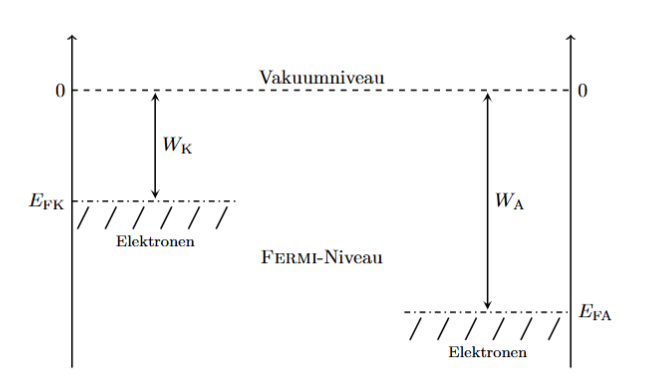
\includegraphics[width=0.75\textwidth]{figs/baenderschema_kathode_anode.png}
    \caption{ Ferminiveaus von Kathode und Anode mit Austrittsarbeit $W_A$ \cite{praktikum}}
    \label{fig:kathode-anode}
\end{figure}
\FloatBarrier

\begin{figure}[htbp]
    \centering
    \includegraphics[width=0.75\textwidth]{figs/anlegen_aeuß_potential.png}
    \caption{ Kontaktpotential $-eU_{KA}$ \cite{praktikum}}
    \label{fig:potential ext}
\end{figure}
\FloatBarrier

\begin{figure}[htbp]
    \centering
    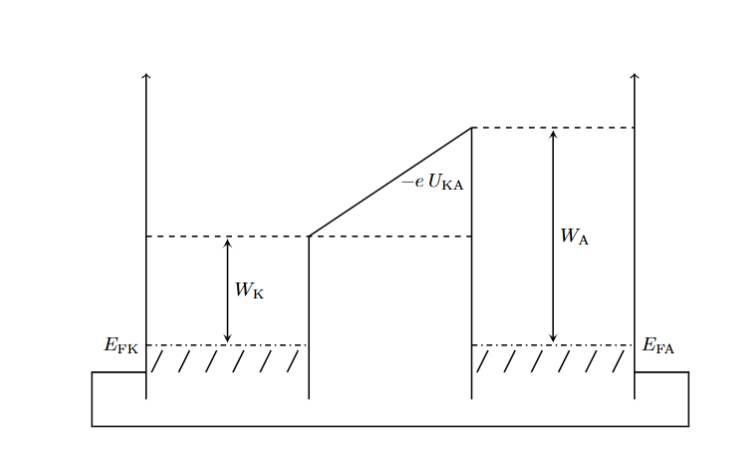
\includegraphics[width=0.75\textwidth]{figs/kontaktpotential_kurzgeschl_elektroden.png}
    \caption{  Potential dass von der Gegenspannung
$-eU_G$ induziert wird\cite{praktikum}}
    \label{fig:potential kurzg.}
\end{figure}
\FloatBarrier


Laut der Abbildung der Ferminiveaus \ref{fig:kathode-anode} 
gilt für die Energiebilanz:
\begin{equation}
    E = h\nu = W_K + eU_{KA} + eU_{G,0} 
    = W_K + W_A - W_K + eU_{G,0} 
    = W_A + eU_{G,0}.
\end{equation}\\
Aus der Frequenz des Lichtes können 
schließlich
die Austrittsarbeit der Anode $W_A$ und 
das Planck’sche Wirkungsquantum h bestimmt 
werden:
\begin{equation}
    eU_{G,0} = h\nu - W_A.
    \label{eq:photoelektrische Gleichung}
\end{equation}
%section{Abschätzung des Plankschen Wirkungsquantums und der Austrittsarbeit}
%\subsection[Bestimmung der Grenzspannung U0]{Bestimmung der Grenzspannung U\textsubscript{0}}
%\subsection[Bestimmung des Plankschen Wirkungsquantums h]{Bestimmung des Plankschen Wirkungsquantums h}

%\subsection[Bestimmung der Austrittsarbeit WA]{Bestimmung der Austrittsarbeit W\textsubscript{A}}

%\subsection[Vergleich der Lambda-Kennlinie für unterschiedliche Intensitäten]{Vergleich der Lambda-Kennlinie für unterschiedliche Intensitäten}
%Diskussionen/Vergleiche werden direkt in den Unterteilen eingebaut
\section{Auswertung}
\cref{eq:photoelektrische Gleichung} stellt eine direkte, quantitative Beziehung zwischen der Energie einfallender Photonen und der kinetischen Energie der von einer Metalloberfläche emittierten Elektronen her. Sie kann geschrieben werden als:

\begin{equation}
    h\,\nu = e\,U_{0} + W_{A},
\end{equation}

wobei $h$ das Plancksche Wirkungsquantum ist, $\nu$ die Lichtfrequenz, $U_{0}$ die Gegenspannung (zur Unterdrückung des Photostroms bis Null), $e$ die Elementarladung ($\equiv \SI{1.602e-19}{\coulomb}$ \cite{codata}) und $W_{A}$ die Austrittsarbeit des Anodenmaterials darstellt. In dieser Formulierung setzt jedes Photon der Energie $h,\nu$ ein Elektron frei, das die Bindungsenergie $W_{A}$ des Materials überwinden muss; jede überschüssige Energie erscheint als kinetische Energie, die elektrisch als $e,U_{0}$ gemessen wird. Diese Gleichung bestätigte nicht nur die Quanten­natur des Lichts, indem sie zeigte, dass der Elektronenaustritt von der Frequenz und nicht der Intensität abhängt, sondern liefert auch eine präzise Methode zur Bestimmung von $h$ und $W_{A}$ anhand experimenteller Messungen von $U_{0}$ in Abhängigkeit von $\nu$.

In unserem Experiment beginnt jeder Messpunkt mit zwei Rohspannungen: der Gegenspannung $U_{G}$, die direkt an dem \SI{100}{\ohm}-Zweig des Spannungsteilers in Millivolt abgelesen wird, und der Photospannung $U_{\mathrm{ph}}$, die der Ausgang des Verstärkers ist und proportional zum Photostrom, ebenfalls in Millivolt. Um die tatsächliche Gegenspannung $U$ zu erhalten, die auf die Elektronen wirkt, wird $U_{G}$ mit $(100+330)/100$ multipliziert, um den Spannungsteiler (\SI{100}{\ohm}:\SI{330}{\ohm}) zu korrigieren. Die Photospannung wird wie folgt in einen Strom umgerechnet: zunächst wird $U_{\mathrm{ph}}$ mit $10^{-3}$ in Volt umgerechnet, dann durch die Verstärkung $G$ (in V/A) geteilt, um $I$ in Ampere zu erhalten, und schließlich mit $10^{12}$ multipliziert, um den Strom in Pikoampere auszudrücken:

\begin{equation}
  U = U_{G}\,\frac{100 + 330}{100},\quad
  I = \frac{U_{\mathrm{ph}}\times10^{-3}}{G}\times10^{12}
  \quad(\mathrm{pA}).
\end{equation}

Durch Anwendung dieser einfachen Einheiten- und Teilerkorrekturen auf jedes $(U_{G},U_{\mathrm{ph}})$-Paar erhalten wir die physikalisch sinnvollen $(U,I)$-Daten, die die Grundlage für die anschließende Linearisierung und Ausgleichsrechnung bilden.

Zur Bestimmung des Sättigungsstroms $I_{0}$ betrachten wir jede Photostromkurve $I(U)$ und bestimmen den Stromwert bei der größten angelegten Gegenspannung $U_{G,\max}$. Physikalisch entspricht dies dem Fall, in dem das Gegenfeld so stark ist, dass dennoch alle emittierten Elektronen zur Anode gelangen – es bildet sich ein Plateau im $I$–$U$-Diagramm. Praktisch bestimmen wir den Index $i$, bei dem $U_{G}$ maximal ist, und definieren:

\begin{equation}
  I_{0} = I\bigl(U = U_{G,\max}\bigr)\quad(\text{in pA}).
\end{equation}

Dieser Einzelwert $I_{0}$ dient dann als Basiswert für die Linearisierung.

Um nun die Gegenspannung $U_{0}$ aus den Messdaten zu extrahieren, bilden wir die transformierte Variable

\begin{equation}
  y = \sqrt{\max\{\,0,\;I(U) - I_{0}\,\}}
\end{equation}

für jeden Punkt der $I$–$U$-Kurve. Wird $y$ gegen die korrigierte Gegenspannung $U$ aufgetragen, ergibt sich im Bereich kurz unterhalb von $U_{0}$ eine nahezu lineare Beziehung, denn theoretisch gilt:

\begin{equation}
  I - I_{0} \;\propto\;(U - U_{0})^{2}.
\end{equation}

Es wird dann eine gewichtete lineare Regression durchgeführt:

\begin{equation}
    y = m \cdot U + b
\end{equation}

unter Verwendung der propagierten Unsicherheiten in $y$ als Gewichte. Die Ausgleichsrechnung liefert die Steigung $m$ und den Achsenabschnitt $b$ mit ihren Standardabweichungen. Der Stoppwert ergibt sich aus der Bedingung $y=0$:

\begin{equation}
  0 = m\,U_{0} + b
  \quad\Longrightarrow\quad
  U_{0} = -\,\frac{b}{m}.
\end{equation}

Durch Fehlerfortpflanzung, einschließlich Kovarianz von $m$ und $b$ (sofern verfügbar), wird ein präziser Wert $U_{0}\pm\sigma_{U_{0}}$ für jede Wellenlänge bestimmt. Diese Gegenspannungen sind die zentralen Größen für das finale Diagramm $U_{0}$ gegen Photonfrequenz, aus dem $h$ und $W_{A}$ extrahiert werden.
\FloatBarrier
\begin{figure}[H]
    \centering
    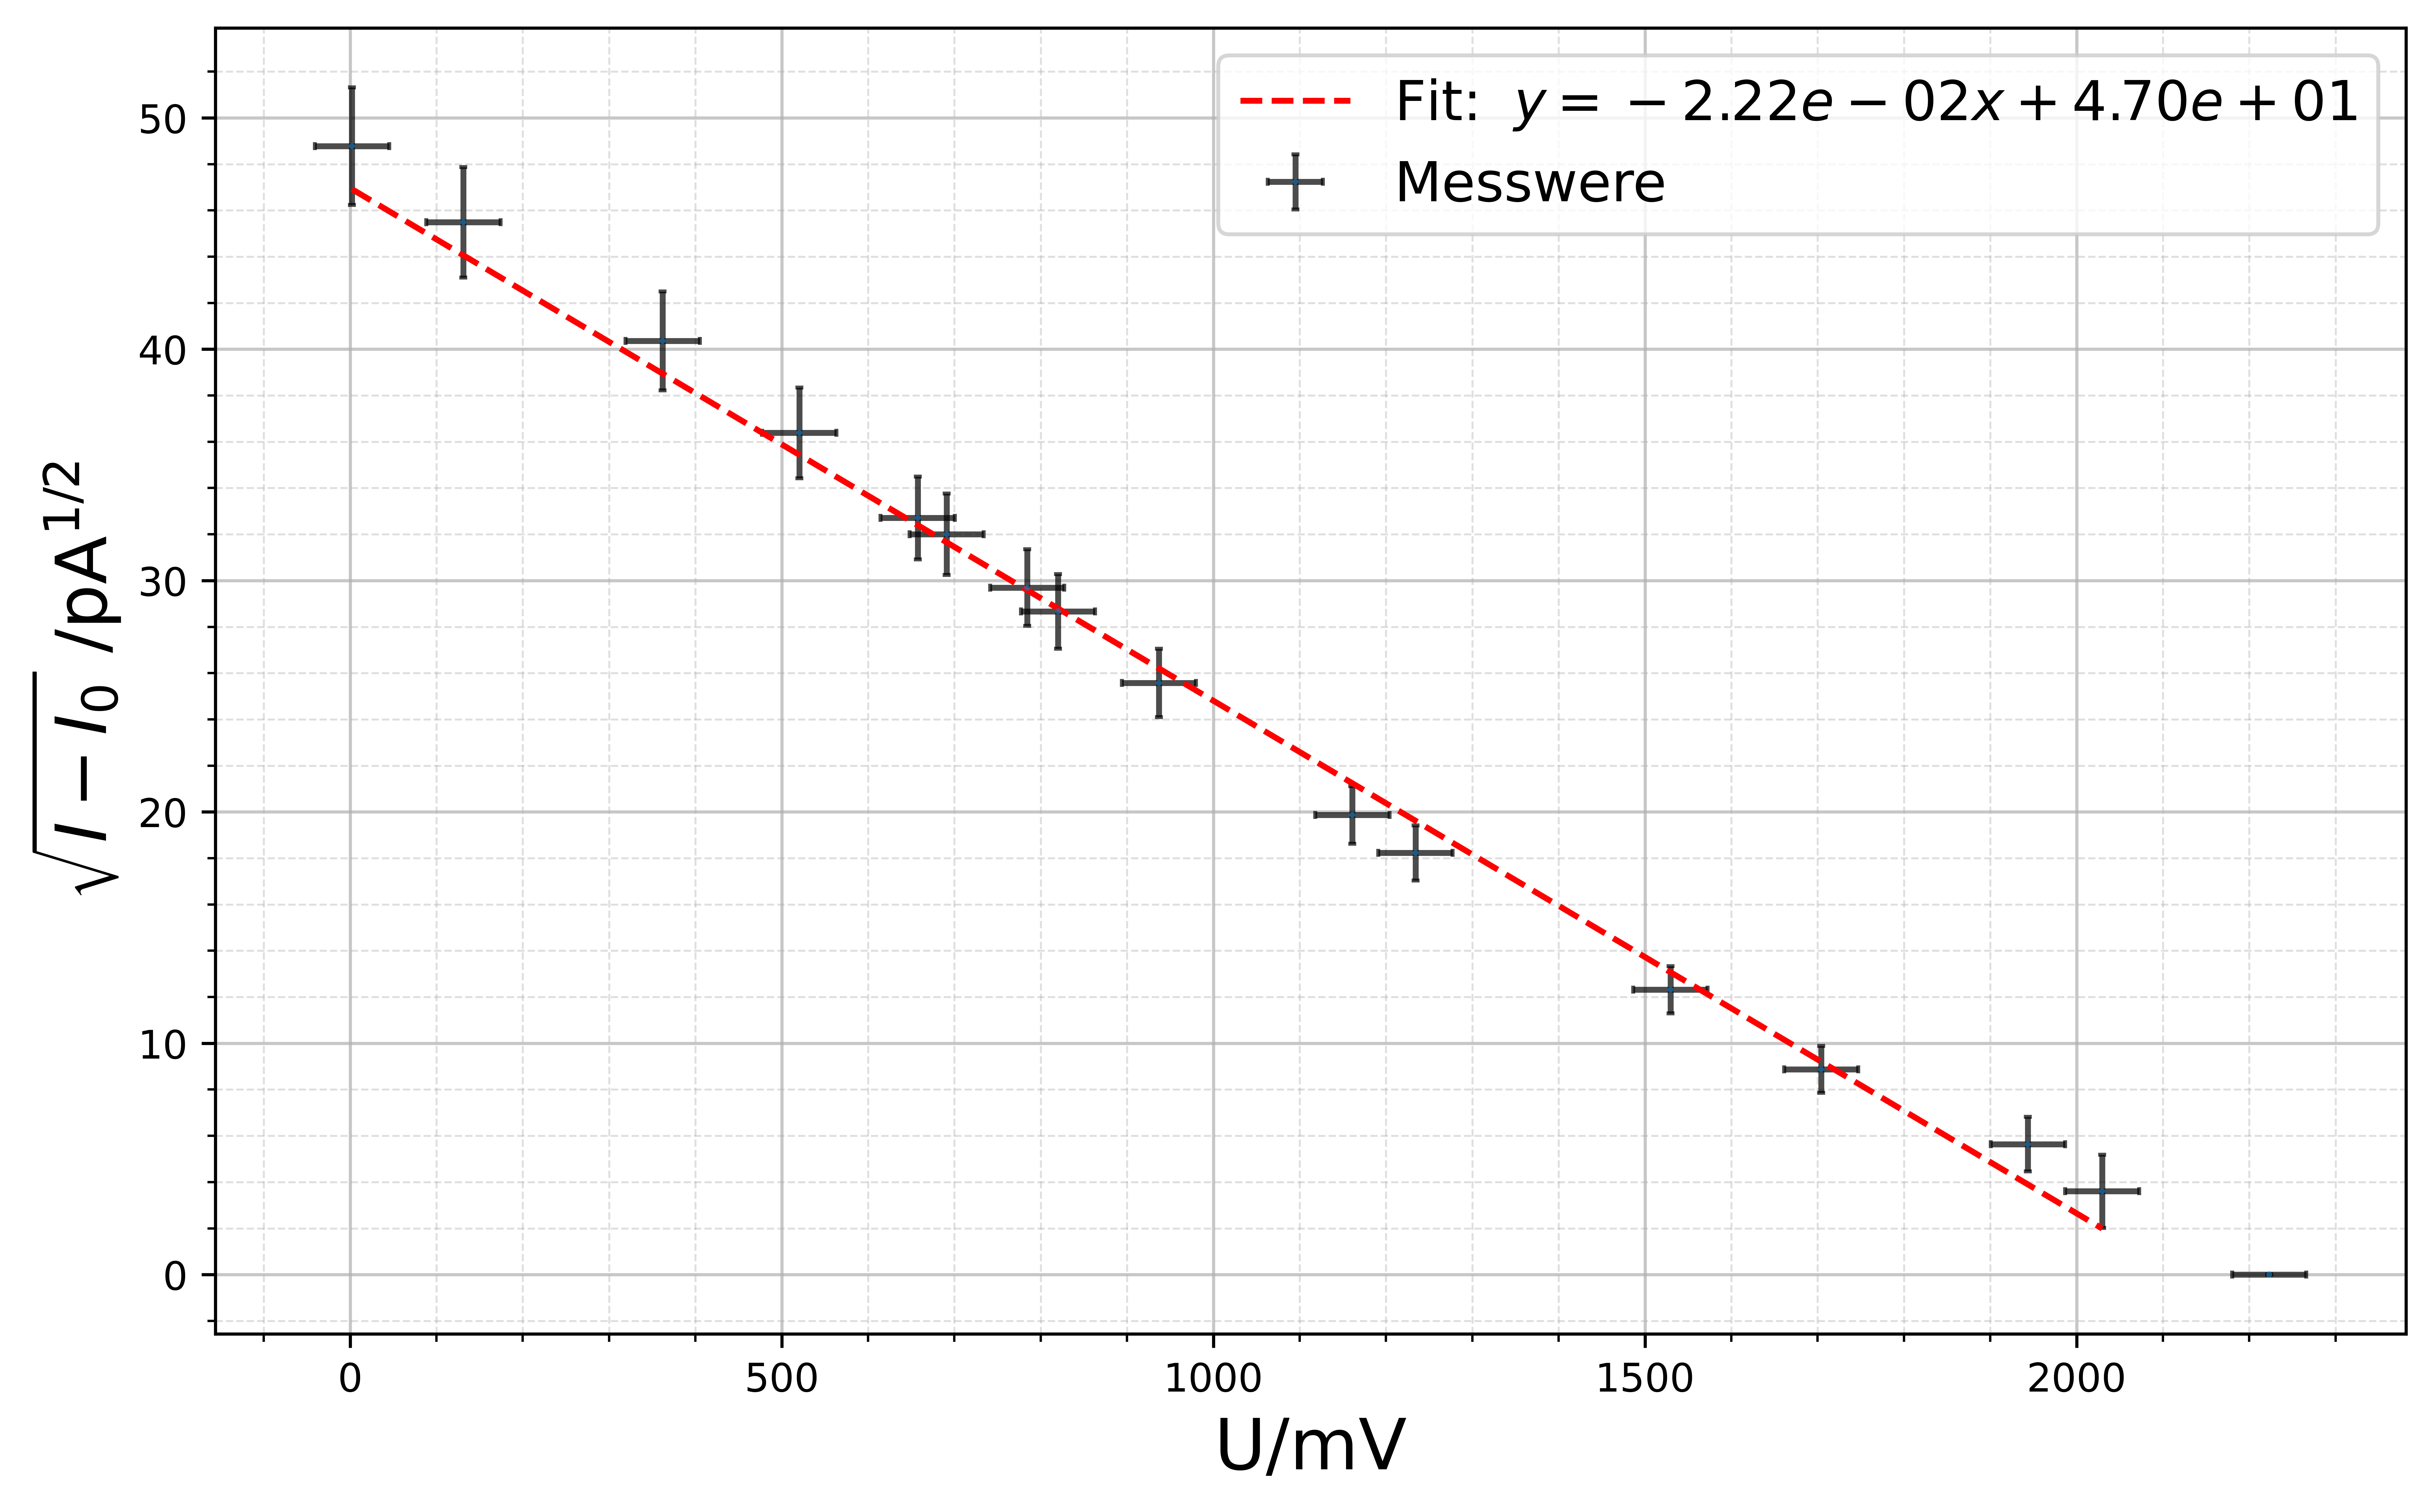
\includegraphics[width=0.95\linewidth]{figs/365_1.png}
    \captionof{figure}{Messung 1 bei $\lambda=\SI{365}{\nm}$. Die Werte und Unsicherheiten sind in ~\cref{tab:365_first}.}
    \label{fig:365_first_photoeff}
\end{figure}
\begin{table}[H]
  \centering
  \begin{tabular}{|c|c|}
    \hline
    \textbf{Parameter} & \textbf{Wert} \\ \hline
    Steigung $m$ [\si{\pico\ampere^{1/2}/\milli\volt}]
      & $\num{-2.22(56)e-2}$ \\ \hline
    Achsenabschnitt $b$ [\si{\pico\ampere^{1/2}}]
      & $\num{4.70(7)e1}$ \\ \hline
    $\chi^2$
      & $\num{8.28}$ \\ \hline
    Freiheitsgrade (dof)
      & $\num{13}$ \\ \hline
    $\chi^2/\mathrm{dof}$
      & $\num{0.64}$ \\ \hline
    Abbremsspannung $U_0$ [\si{\milli\volt}]
      & $\num{2117.12 \pm 62.98}$ \\ \hline
  \end{tabular}
  \caption{Ergebnisse des gewichteten linearen $\chi^2$-Fits zur Bestimmung der Abbremsspannung für die erste Messung bei $\lambda=\SI{365}{\nano\metre}$. Die hier gezeigten Werte stammen aus Tabelle~\ref{tab:365_first}.}
  \label{tab:365_first_chi2_photoeff}
\end{table}
\FloatBarrier
Aus dem \cref{fig:365_first_photoeff} und der \cref{tab:365_first_chi2_photoeff} ergibt sich für die erste Messung bei $\lambda = \SI{365}{\nano\meter}$ eine Stoppspannung von $U_0 = \SI{2117.12 \pm 62.98}{\milli\volt}.$ Weitere Diagramme für unterschiedliche Wellenlängen befinden sich im Anhang zwischen \cref{fig:365_first} und \cref{fig:578_second}, die zugehörigen Tabellen zwischen \cref{tab:365_first} und \cref{tab:578_second}.\\



Da die Photonenergie $E$ direkt proportional zur Frequenz ist über $E = h\nu$, muss jede zentrale Filterwellenlänge $\lambda$ in die entsprechende Frequenz $\nu$ umgerechnet werden. Im Vakuum gilt:

\begin{equation}
    \nu = \frac{c}{\lambda},
\end{equation}

wobei $c$ die Lichtgeschwindigkeit ist ($= \SI{299 792 458}{\metre\per\second}$ \cite{codata}) und $\lambda$ in Metern angegeben wird.

In unserem Versuch wurde jede Wellenlänge zweimal gemessen, was zwei Stoppspannungen $U_{0,1}$ und $U_{0,2}$ ergibt. Deren gewichteter Mittelwert ist:

\begin{equation}
  \begin{aligned}
    \mathrm{inv\_var}_1 &= \frac{1}{\sigma_{1}^{2}},\quad
    \mathrm{inv\_var}_2 = \frac{1}{\sigma_{2}^{2}},\\[1ex]
    U_{0,\mathrm{avg}}  &= \frac{U_{0,1}\,\mathrm{inv\_var}_1 + U_{0,2}\,\mathrm{inv\_var}_2}
                               {\mathrm{inv\_var}_1 + \mathrm{inv\_var}_2},\\[1ex]
    \sigma_{0,\mathrm{avg}} &= \sqrt{\frac{1}{\mathrm{inv\_var}_1 + \mathrm{inv\_var}_2}}.
  \end{aligned}
\end{equation}

Die so gemittelten Stoppspannungen $U_{0,\mathrm{avg}}$ (in Millivolt) werden gegen die entsprechenden Frequenzen $\nu$ (in Hertz) aufgetragen (\cref{fig:fvsU}), um Einsteins Vorhersage zu überprüfen:

\begin{equation}
  e\,U_{0} = h\,\nu - W_{A}.
\end{equation}

Umgeschrieben nach $U_{0}$ ergibt sich die lineare Form:

\begin{equation}
  U_{0} = \frac{h}{e}\,\nu - \frac{W_{A}}{e}.
\end{equation}
\FloatBarrier
\begin{figure}[H] 
  \centering
  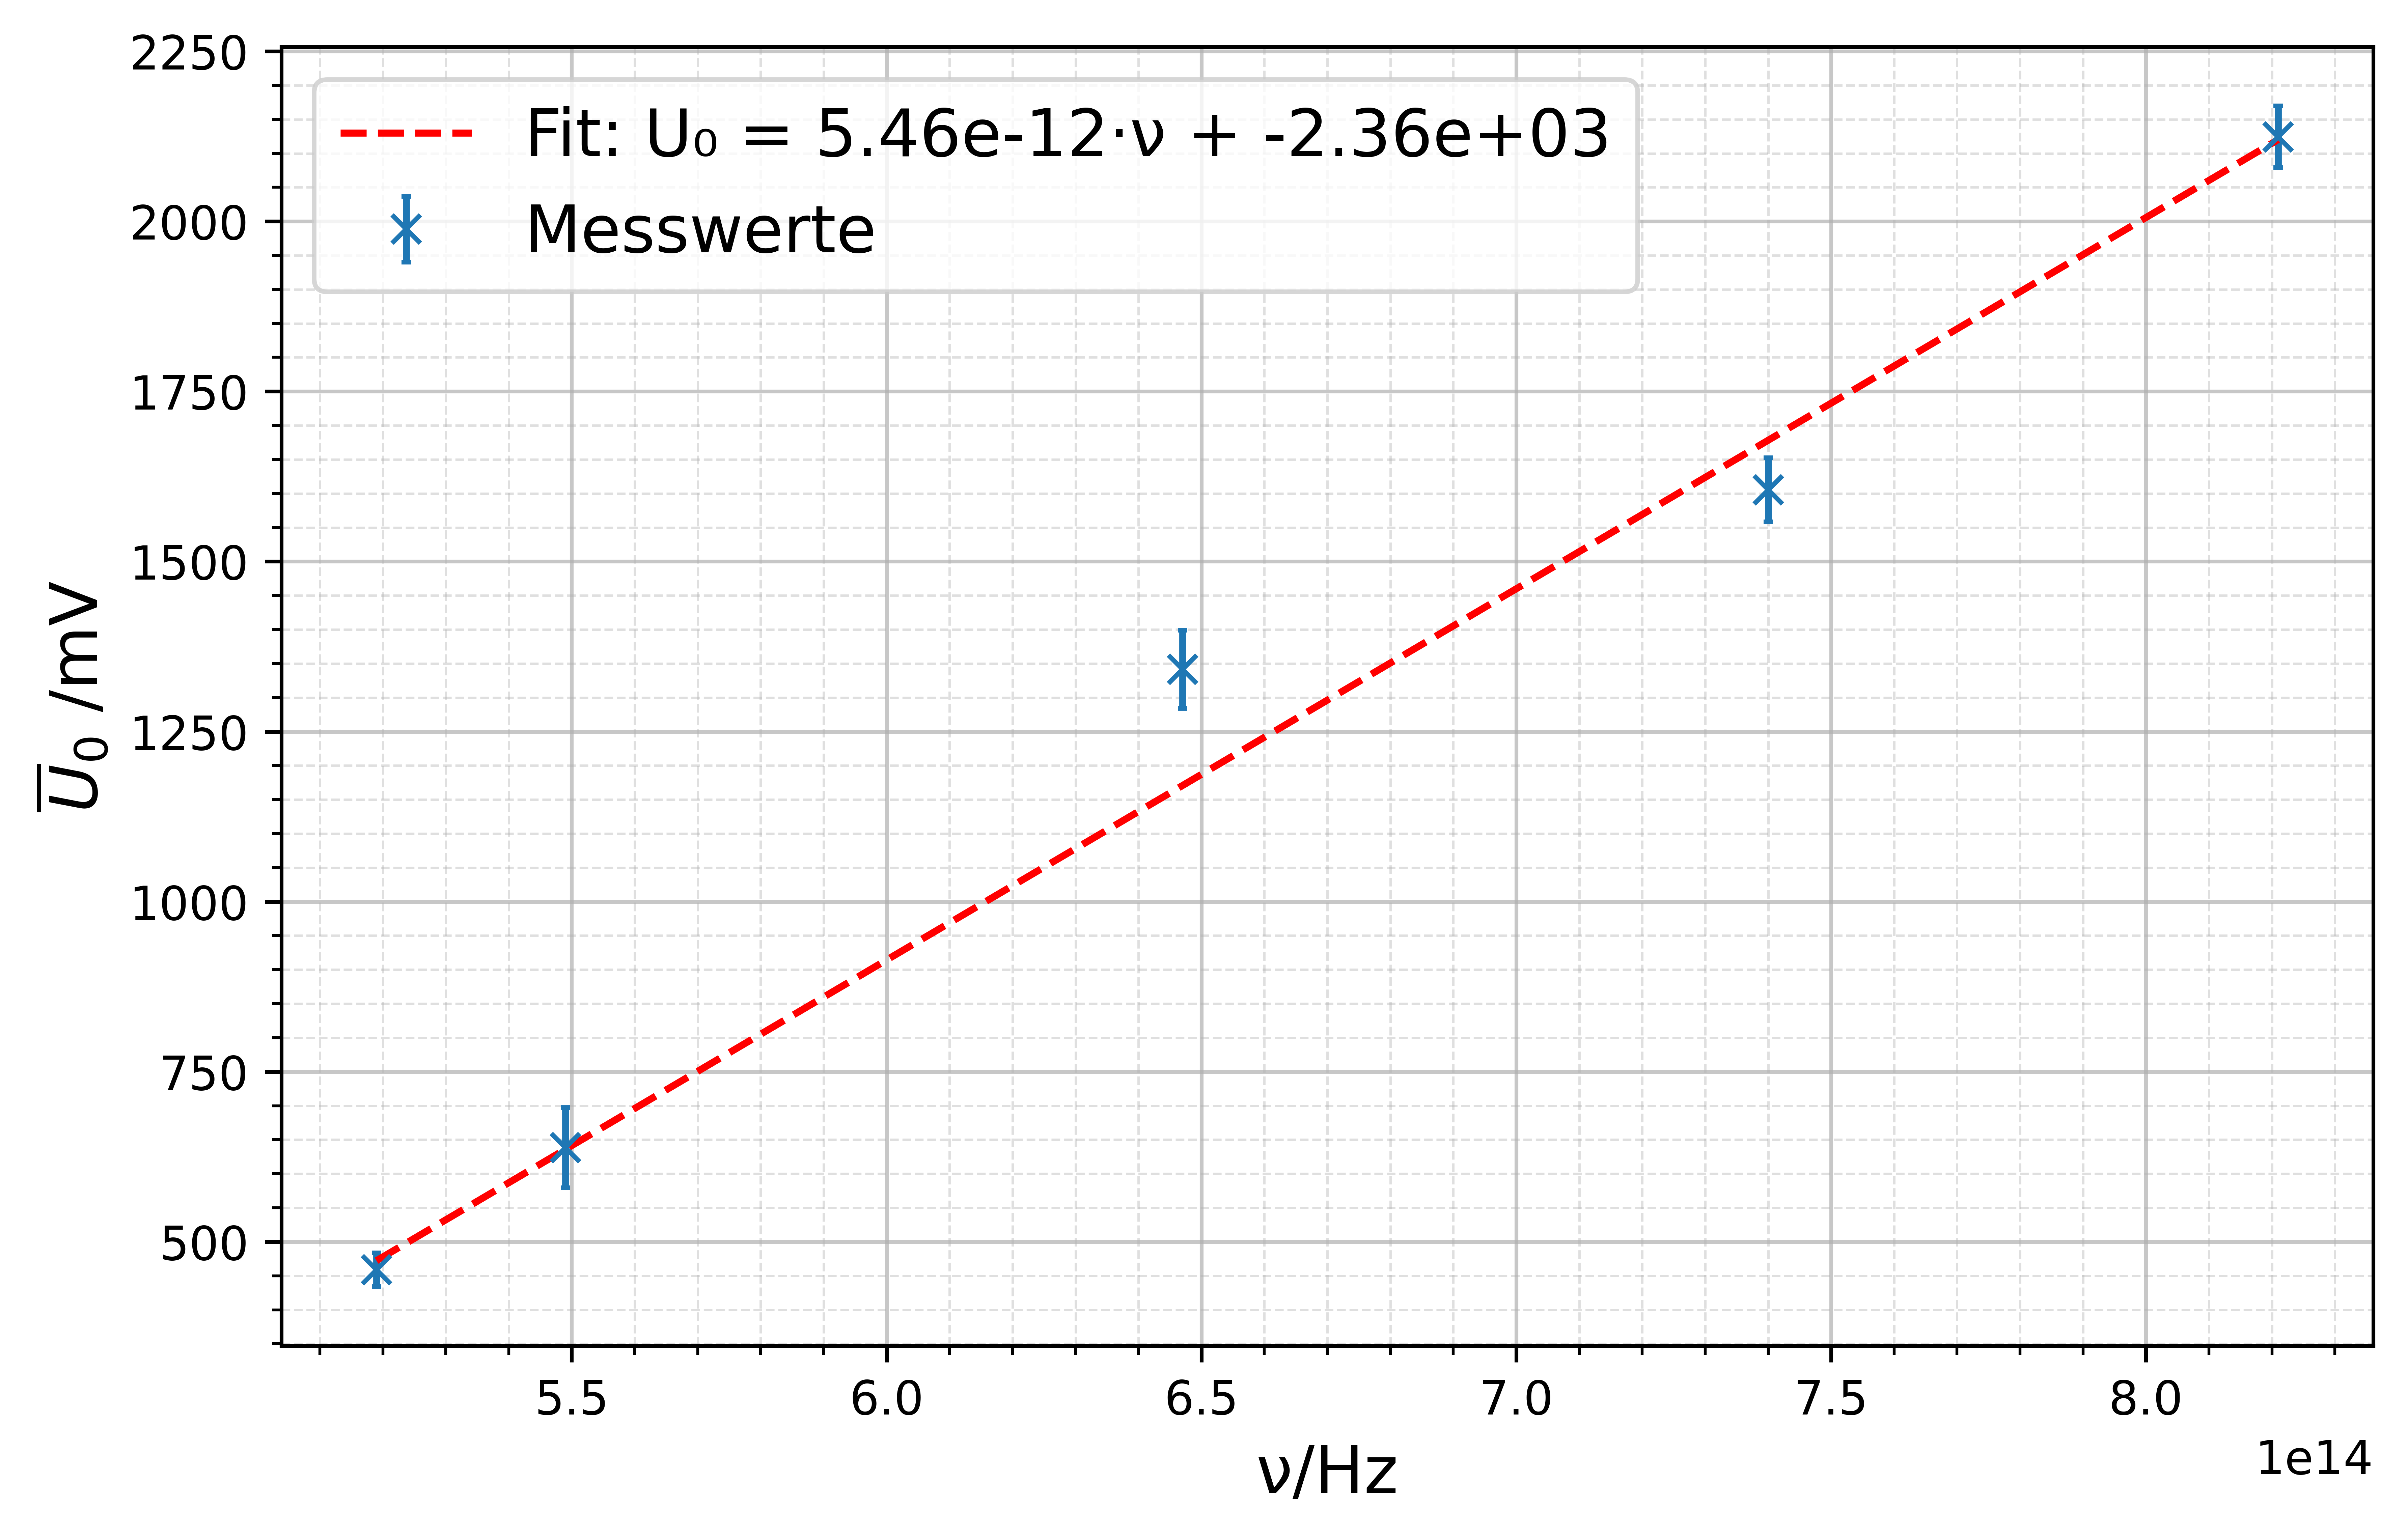
\includegraphics[width=0.95\linewidth]{figs/fvsU.png}
  \captionof{figure}{Gemittelte Stoppspannungen $U_0$ gegen Frequenzen $\nu$. Werte und Unsicherheiten sind in \cref{tab:U0_vs_nu_data} angegeben.}
  \label{fig:fvsU}
\end{figure}
\begin{table}[H]
\centering
\resizebox{0.75\columnwidth}{!}{%
\begin{tabular}{|c|c|c|c|}
\hline
$\lambda$ [\si{\nano\metre}] & $\nu$ [\si{\hertz}] & $\overline{U_0}$ [\si{\milli\volt}] & $\Delta \overline{U_0}$ [\si{\milli\volt}] \\ \hline
\SI{365.00}{\nano\metre} & \num{8.21e14} & \num{2124.19} & \num{45.39} \\ \hline
\SI{405.00}{\nano\metre} & \num{7.40e14} & \num{1605.23} & \num{47.04} \\ \hline
\SI{463.00}{\nano\metre} & \num{6.47e14} & \num{1341.51} & \num{57.42} \\ \hline
\SI{546.00}{\nano\metre} & \num{5.49e14} & \num{638.22}  & \num{59.13} \\ \hline
\SI{578.00}{\nano\metre} & \num{5.19e14} & \num{458.70}  & \num{24.80} \\ \hline
\end{tabular}%
}
\caption{Gemittelte Abbrems­spannungen $\overline{U_0}$ und deren Unsicherheiten gegen die jeweiligen Frequenzen.}
\label{tab:U0_vs_nu_data}
\end{table}

\begin{table}[H]
\centering
\resizebox{0.75\columnwidth}{!}{%
\begin{tabular}{|c|c|}
\hline
\textbf{Parameter} & \textbf{Wert} \\ \hline
Steigung $m$ [\si{\milli\volt\per\hertz}] 
  & $\num{5.46e-12} \pm \num{2.95e-13}$ \\ \hline
Achsenabschnitt $b$ [\si{\milli\volt}] 
  & $\num{-2.36e3} \pm \num{1.84e2}$ \\ \hline
$\mathrm{\chi}^2$ 
  & $\num{11.56}$ \\ \hline
Freiheitsgrade (dof) 
  & 3 \\ \hline
$\mathrm{\chi}^2 / \mathrm{dof}$ 
  & $\num{3.85}$ \\ \hline
\end{tabular}%
}
\caption{Ergebnisse des gewichteten linearen $\mathrm{\chi}^2$-Fits von $\overline{U_0}$ gegen $\nu$.}
\label{tab:U0_vs_nu_fit}
\end{table}
\FloatBarrier

Ein linearer Fit von $U_{0,\mathrm{avg}}(\nu)$ (\cref{fig:fvsU})hat also die Steigung $m = h/e$ und den y-Achsenabschnitt $b = -W_{A}/e$ (Werte in \cref{tab:U0_vs_nu_fit}). Daraus ergibt sich:


\begin{equation}
  h = m\,e,
\end{equation}

sowie die Austrittsarbeit der Anode:

\begin{equation}
  W_{A} = -\,b\,e,
\end{equation}

die durch Division durch $e$ in Elektronenvolt umgerechnet wird. Numerisch ergibt sich:

\begin{equation}
\begin{split}
  h &= \bigl(5.457\times10^{-12}\,\mathrm{mV/Hz}\bigr)\;\times\;\frac{1.602\times10^{-19}\,\mathrm{C}}{10^3}\\
    &\Longrightarrow\;8.74\times10^{-34}\,\mathrm{J\cdot s}\;\pm\;4.7\times10^{-35}\,\mathrm{J\cdot s}
\end{split}
\end{equation}

\begin{equation}
\begin{split}
  W_{A} &= -\bigl(-2.360\times10^{3}\bigr)\;\times\;\frac{1.602\times10^{-19}\,\mathrm{C}}{10^3}\\
        &\Longrightarrow\;3.78\times10^{-19}\,\mathrm{J}
         \;\Longrightarrow\;2.36\,\mathrm{eV}\;\pm\;0.18\,\mathrm{eV}
\end{split}
\end{equation}

Diese experimentell bestimmten Werte für $h$ und $W_{A}$ werden abschließend mit dem CODATA-Wert $h=\SI{6.626 070 15e-34}{J.s}$ \cite{codata}.

%\section*{Diskussion und Fehleranalyse}

Unser berechneter Wert für das Plancksche Wirkungsquantum liegt etwa 32\,\% über dem anerkannten CODATA-Wert von. Diese systematische Überschätzung deutet darauf hin, dass - obwohl unsere lineare Ausgleichsrechnung der Stoppspannung gegen die Frequenz intern konsistent war (\(\chi^2/\mathrm{dof}\approx3{,}8\)) - gewisse Kalibrierungs- oder Justierfehler bestehen geblieben sind.

Die bestimm­te Austrittsarbeit der Anode lässt sich nicht direkt mit Literaturwerten vergleichen, da Material
und Zustand der Kathode/Anode in der verwendeten Einweg-Photodiode nicht
bekannt sind.

\paragraph{Fehlerquellen und zukünftige Verbesserungen}

\begin{itemize}
  \item \textbf{Spannungskalibrierung:} Spannungsteiler und Messverstärker führen zu
    Skalierungsunsicherheiten. Zukünftig sollten 0{,}1\,\%-Präzisionswiderstände
    und ein kalibriertes Digitalvoltmeter verwendet werden.

  \item \textbf{Drift des Photostromverstärkers:} Temperaturschwankungen beeinflussen
    die Transimpedanzverstärkung. Eine Temperaturstabilisierung oder regelmäßige
    Nullpunktnachführung während der Messung ist empfehlenswert.

  \item \textbf{Kontaktpotenzial und Dunkelstrom:} Oberflächeninhomogenitäten und
    Leckströme können \(U_0\) systematisch verfälschen. Eine Ausheizung und
    Abschirmung der Photodiode sowie die Vorabmessung des Dunkelstroms sind
    hilfreich.

  \item \textbf{Ausrichtung und Fokussierung:} Eine ungleichmäßige Beleuchtung durch
    falsche Fokussierung kann Messfehler verursachen. Eine fein verstellbare
    optische Plattform und Kamerabeobachtung des Fokusflecks sind hier sinnvoll.
\end{itemize}
\paragraph{Intensitätsabhängigkeit bei $\lambda = \SI{365}{\nano\meter}$} :
Wir untersuchten die Stoppspannung $U_0$ bei zwei unterschiedlichen Lichtintensitäten – etwa 50\,\% und maximaler Lampenleistung – unter ansonsten identischen Versuchsbedingungen.

Bei 50\,\% Intensität ergaben die Messdaten einen Plateau-Photostrom von
\begin{equation}
  I_0 = \bigl(10{,}00 \pm 11{,}00\bigr)\,\mathrm{pA},
\end{equation}
und aus dem gewichteten Fit von $\sqrt{I - I_0}$ gegen $U$ eine Stoppspannung von
\begin{equation}
  U_0(50\,\%) = \bigl(2136{,}2 \pm 92{,}0\bigr)\,\mathrm{mV}
  \quad\bigl(\chi^2/\mathrm{dof} = 0{,}82\bigr).
\end{equation}

Bei voller Intensität stieg der Plateau-Strom auf
\begin{equation}
  I_0 = \bigl(1{,}50 \pm 10{,}15\bigr)\,\mathrm{pA},
\end{equation}
(anmerkend, dass das Vorzeichen aufgrund der umgekehrten $\lambda$–$U$-Reihenfolge wechselt), und der Fit ergab:
\begin{equation}
  U_0(100\,\%) = \bigl(2190{,}0 \pm 108{,}4\bigr)\,\mathrm{mV}
  \quad\bigl(\chi^2/\mathrm{dof} = 1{,}47\bigr).
\end{equation}

Diese beiden Werte für $U_0$ stimmen innerhalb ihrer jeweiligen $1\sigma$-Unsicherheiten überein und bestätigen Einsteins Vorhersage, dass die Stoppspannung nur von der Frequenz der Photonen abhängt – nicht jedoch von der Intensität des einfallenden Lichts. Die Plateau-Ströme $I_0$ hingegen skalieren erwartungsgemäß mit der Lichtintensität. Graphen sind in \cref{fig:365_50} und \cref{fig:365_max} dargestellt und Werte in \cref{tab:365_50pct} und \cref{tab:365_max}.

\subsection*{Mögliche Ursachen für verbleibende Abweichungen}
\begin{itemize}
  \item Unsicherheit bei der exakten Einstellung der Blende auf 50\,\% sowie Lampendrift über die Zeit,
  \item Offset-Drift des Photostromverstärkers zwischen den Messreihen,
  \item Leichte Fehljustierung oder Fokusschwankungen beim Ändern der Intensität,
  \item Statistische Streuung im Bereich kleiner Ströme nahe der Abschneide­spannung.
\end{itemize}

\subsection*{Empfehlungen zur Optimierung künftiger Messungen}
\begin{itemize}
  \item Stabilisierung der Lampenleistung mittels geregeltem Netzteil,
  \item Verwendung eines automatisierten Graufilterrades zur präzisen Intensitätsregelung,
  \item Temperaturstabilisierung von Verstärker und Fotozelle,
  \item Erfassung zusätzlicher Messpunkte nahe der Cutoff-Region zur Reduktion der Fit-Unsicherheit.
\end{itemize}
